\section{Datenbankstruktur}

Alle Daten werden in einer MySQL-Datenbank gespeichert. Das ER-Diagramm ist wie folgt: 

\begin{figure}[ht]
	\centering
	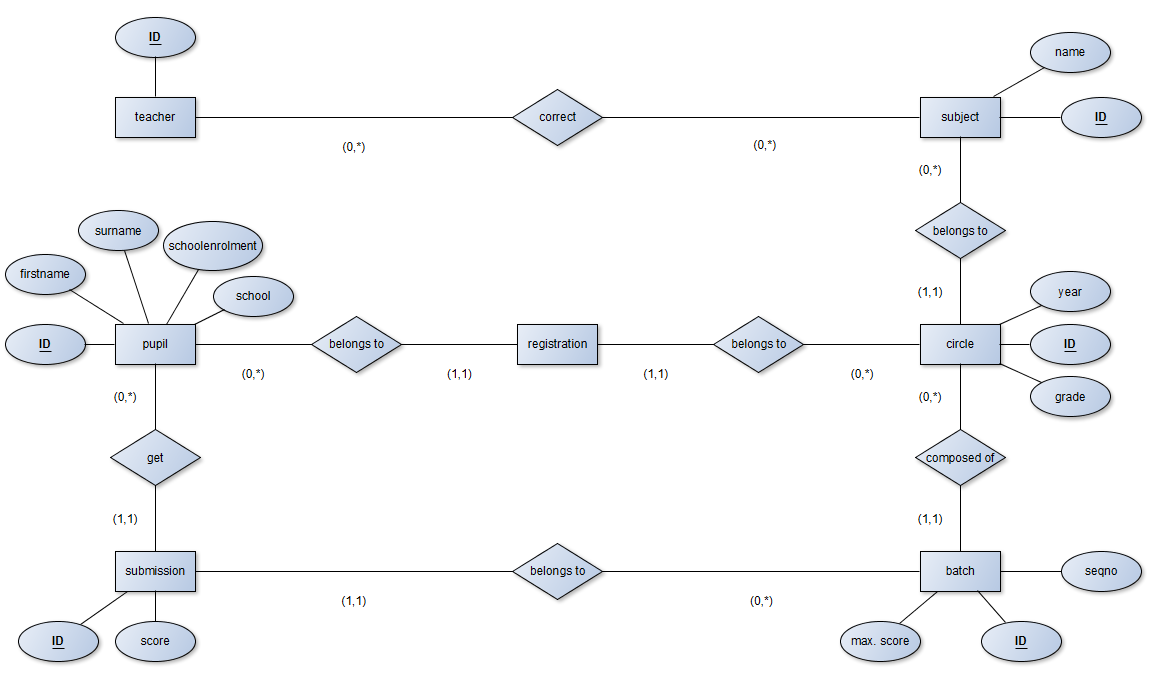
\includegraphics[scale=.50]{bilder/ER-Modell_engl.PNG}
	\caption{ER-Diagramm}
	\label{abb:beispiel}
\end{figure}

Es wurden für alle Datenbankelemente englische Begriffe verwendet, um das Programmieren zu erleichtern. So muss häufig zwischen Einzahl und Mehrzahl unterschieden werden, was bei deutschen Begriffen zum Teil unmöglich ist (Einzahl: "`Schüler"'; Mehrzahl: "`Schüler'").

Die Umsetzung des ER-Diagramms erfolgt mittels "`Laravel"': über sogenannte "`Migrationen"' wird dort festgelegt, wie Tabellen, Spalten und Fremdschlüssel automatisch erzeugt werden.